\documentclass{report}
\usepackage{amsfonts}
\usepackage{amssymb}
\usepackage{amsmath}
\usepackage{amsthm}
\usepackage{hyperref}
\usepackage[a4paper, margin=1in]{geometry}
\usepackage{algorithm}
\usepackage{algpseudocode}
\usepackage{caption}
\usepackage{graphicx}


\DeclareCaptionFormat{myformat}{#3}
\captionsetup[algorithm]{format=myformat}
\algnewcommand{\LineComment}[1]{\State{\(\triangleright\) #1}}

\DeclareMathOperator{\argmin}{argmin}

\newtheorem{defin}{Definition}[chapter] 
\newtheorem{prop}{Proposition}[chapter] 
\newtheorem{teo}{Theorem}[chapter] 
\newtheorem{es}{Exercise example}[chapter] 

\title{Data Organization}
\author{Martino Papa}
\date{19 march 2025}
\begin{document}
\maketitle
\tableofcontents

\chapter*{Introduction}
In 2020 the \textit{Digital Universe Study of International Data Corporation} estemed that humanity have stored 40ZB of data, corrisponding to 5247 GB per person. Only 1\% of those data has been analysed due to the high presence of desctructureted data. \textbf{Big data analytics} consists in using sophisticated techniques on a big amount of data with the goal of describing events, situations, identyfing patterns and finding correaltions. There are 4 different types of data analytics:
\begin{itemize}
    \item descreptive analysis, understanding what happend;
    \item predictive analysis, predicting what's going to happend;
    \item prescreptive analysis, understanding how to react to a certain event;
    \item diagnostical analysis, understanding why something happend.
\end{itemize}
In the Big data analytics there are 3 main problems known as the “three V”.
\begin{itemize}
    \item volume, the enormus amount of data bring problems to memorization and analysis;
    \item velocity, the amount of new data makes them difficoult to process online;
    \item varaiety, different types of data are difficoult to handle.
\end{itemize}
\chapter{Memory hierarchy}
In a computer the data can be stored in different types of memories with different goals. In order to be processed from the CPU data needs to be in the CPU registers, whose are fast but also very small thus we need to store all the data somplace else. There are different types of memories, the bigger they get the slower they will be. All the data are stored in the biggest one and then they are moved to the smaller ones when they need to be processed.
The memories inside a computer listed from the slowest and biggest to the fastest and smallest are the following.
\begin{itemize}
    \item External Memory (EM)
    \item Random Access Memory (RAM)
    \item Cache
    \item CPU registers
\end{itemize}
Usually in algorithms complexity analysis all memory access are treated as they would take the same time. In fact if an algorithm has to work on different machines we cannot refer to a specific structure.
To imporve the performance Operating Systems choose where to store the data following two principles.
\begin{prop}[Locality of Time]
    If a program accesses certain memory locations, it is likely to access the same locations again in the near future.
\end{prop}
\begin{prop}[Locality of Space]
    If a program accesses a particular memory location, it is likely to access nearby memory locations soon after.
\end{prop}
\noindent
When we move data two the faster memories we count on the fact that Locality of Time tells that they are probably gonna be needed again. To profit by Locality of Space the data are moved in blocks. \\
When an access to a location \textit{l} is required the computer proceeds as follows:
\begin{algorithm}[H]
    \begin{algorithmic}[1]
    \LineComment{the CPU determines if \(\textit{l}\) is in the cache}
    \If{\textit{l} is in the cache}
    \LineComment{the CPU access \textit{l} and goes two the next instruction}
    \Else{}
    \LineComment{the block \(b\) of EM containing \textit{l} is moved in the cache}
    \EndIf{}
    \end{algorithmic}
\end{algorithm}
\noindent
When a block \(b\) is moved if the cache is already full one block has to be removed in regard to load \(b\). To choose which block two remove there are differents possible strategies.
\begin{itemize}
    \item \textbf{Random choice}. Easy to implement, the cost is constant but locality of time and space aren't used.
    \item \textbf{First In First Out (FIFO)}. Easy to implement with a queue, the cost is constant, tries to profit by Locality of Time.
    \item \textbf{Least Frequently Used (LFU)}. Implemented with a priority queue based on the number of accesses to every block. Tries to profit by both Time and Space Locality but it penalizes recently added blocks.
    \item \textbf{Least Recently Used (LRU)}. Implemented with a priority queue with locators (references that allow efficient accesses). High implementation cost. Very efficient, priors mostly by Locality of Time.
    \item \textbf{Marker}. A boolean value \textbf{marked} initialized to \textit{False} is assigned to each block in the cache, when the program access a block it sets \textbf{marked}=\textit{True}. When a block needs to be removed a random one having \textbf{marked}=\textit{False} is choosen. Once every block in the cache has value \textit{True} they all change to \textit{False}. 
\end{itemize}
\paragraph{Competitive analysis of the strategies} To analyse how good a strategy is we compare it to a theoretical optimal one.
\begin{defin}[On-line algorithm]
    They perform on an unknown set of requests with different costs.
\end{defin}
\begin{defin}[Off-line algorithm]
    They perform on a pre-known set of requests.
\end{defin}
\noindent
Competitive analysis consists in confronting on-line algorithms with an optimal off-line one.
\begin{defin}[c-competitivie algorithm]
    Let \(\textsf{OPT}\) be the optimal off-line algorithm, \(A\) an on-line algorithm, \(P=(P_1,\dots,P_n)\) a sequence of instructions. We say that \(A\) is c-competitivie, \(c \geq 0\) if 
    \begin{equation}
        \text{cost}(A,P) \leq c \cdot \text{cost}(\textsf{OPT}, P) + b,\; b\geq 0
    \end{equation}
    c is defined as competitive factor of \(A\).
\end{defin}
\begin{prop}
    FIFO and LRU strategies are \(m\)-competitive with \(m\) number of blocks in the cache.
\end{prop}
\noindent
An on-line randomised algorithm can have different executions on the same sequence of instructions, in this case we say that is \(c\)-competitive if 
\begin{equation}
    \mathbb{E}[\text{cost}(A,P)] \leq c \cdot \text{cost}(\textsf{OPT}, P) + b,\; b\geq 0
\end{equation}
\begin{prop}
    Marker strategy has a competitive factor \(O(\log m)\), with m beeing the number of blocks in the cache.
\end{prop}
\section{Computational models}
\begin{defin}[Architectual model]
    The architectual model represents the essential components involved in the execution of algorithms.
\end{defin}
\begin{defin}[Programming model]
    The programming model specifies the set of instructions used to describe algorithms.
\end{defin}
\begin{defin}[Cost model]
    The cost model defines functions that mesure how good algorithms' performances are.
\end{defin}
\noindent
The model that is usuallly used in analysis of algorithms and data structures is called \textbf{RAM model} and it's defined as follows.
\begin{itemize}
    \item The architectual model consists in a RAM memory and a CPU.
    \item The programming model describes arithmetic, logic, reading, confronts and writing operations.
    \item The cost model defines the \textit{time cost} as the number of operations that an algorithm requires, and the \textit{space cost} as the number of used memory cells. 
\end{itemize}
The model assumes that every reading and writing operation has a constant cost. This is not true with \textit{big dimension problems}.
\begin{defin}[Big dimension problem]
    A problem is called \textit{big dimension problem} if the dimension of the input data is bigger than the dimension of the system's memory.
\end{defin}
\noindent
To handle those problem we introduce an external memory. Those type of memory are much bigger but slower, the assumption that every reading and writing operation has a constant cost falls. Thus we replace the RAM model with a new model called \textbf{Disk model}.
\begin{itemize}
    \item The architectual model consists in a CPU a RAM memory and an External Memory.
    \item The programming model describes, on top of the operation described in the RAM model, operations of input/output regarding the EM.
    \item The cost model defines two functions:
    \begin{itemize}
        \item Work \(W(N,M,B)\), number of elementar operations;
        \item Transfer \(T(N,M,B)\), number of I/O operations.
    \end{itemize}
\end{itemize}
Where \(N\) is the dimension of the problem (number of datapoints), \(M\) the dimension of the internal memory (RAM), \(B\) dimension of transferd blocks (\textbf{pages}), \(Q\) number of interrogations to the memories and \(Z\) is the dimension of each answer. Referring to the number of needed blocks we also define 
\[
    n = \frac{N}{B},\; m=\frac{M}{B}, \; z = \frac{Z}{B}
\]
With this notation we can analise how much fundamental operations cost in terms of Transfer.
\begin{itemize}
    \item SCAN(\(N\)), scanning a file of N elements takes \(\Theta (\frac{N}{B}) = \Theta (n)\) I/O operations.
    \item SORT(\(N\)), sorting a file of N elements takes \(\Theta (n \log_m n)\) I/O operations.
    \item SEARCH(\(N\)), searching in file of N sorted elements takes \(\Theta(\log_B n)\), \(\Theta(1)\) with hash sets I/O operations.
    \item OUTPUT(\(Z\)), returning \(Z\) elemnts output of a query takes \(\Theta(\max \{1,z\})\) output operations.
\end{itemize}
\chapter{Sorting on External Memories}
The problem of sorting a set \(S\) consisting in \(N\) records memorised in External Memory can be firstly approached using the known algorithms used in central memory. Let's suppose that \(S\) is memorised in continuos postion of the EM, one of the most used algorithms in central memory is \textbf{Mergesort}.
\begin{algorithm}[H]
    \caption{MergeSort(\(A, left, right\))}
    \begin{algorithmic}[1]
    \If{\(left < right\)}
        \State \(mid \gets \lfloor (left + right) / 2 \rfloor\)
        \State \textsc{MergeSort}(\(A, left, mid\))
        \State \textsc{MergeSort}(\(A, mid + 1, right\))
        \State \textsc{Merge}(\(A, left, mid, right\))
    \EndIf
    \end{algorithmic}
\end{algorithm}

\begin{algorithm}[H]
    \caption{Merge(\(A, left, mid, right\))}
    \begin{algorithmic}[1]
    \State \(n1 \gets mid - left + 1\), \(n2 \gets right - mid\)
    
    \For{\(i \gets 1\) to \(n1\)}
        \State \(L[i] \gets A[left + i - 1]\)
    \EndFor
    \For{\(j \gets 1\) to \(n2\)}
        \State \(R[j] \gets A[mid + j]\)
    \EndFor
    
    \State \(i \gets 1, j \gets 1, k \gets left\)
    \While{\(i \leq n1\) \textbf{and} \(j \leq n2\)}
        \If{\(L[i] \leq R[j]\)}
            \State \(A[k] \gets L[i]\)
            \State \(i \gets i + 1\)
        \Else
            \State \(A[k] \gets R[j]\)
            \State \(j \gets j + 1\)
        \EndIf
        \State \(k \gets k + 1\)
    \EndWhile
    
    \While{\(i \leq n1\)}
        \State \(A[k] \gets L[i]\)
        \State \(i \gets i + 1, k \gets k + 1\)
    \EndWhile
    
    \While{\(j \leq n2\)}
        \State \(A[k] \gets R[j]\)
        \State \(j \gets j + 1, k \gets k + 1\)
    \EndWhile
    \end{algorithmic}
\end{algorithm}
\noindent
The algorithm divides recursively the set in two halfs untill it contains a single element, then the merge procedure joins two sorted half of dimension \(n_1,n_2\) in \(O(n_1 + n_2)\) time. The algorithm works in \(\Theta(n \log n)\) time and \(\Theta(n)\) space. The problem is that it's not efficient in EM because it requires a lot of I/O operations. Mergesort is translated in the Disk Model with parameters \(M, B\) and \(N\) lenght of \(S\) by the algorithm 2-Mergesort defined as follows.   
\begin{algorithm}[H]
    \caption{2-Mergesort(\(S\), \(N\), \(M\), \(B\))}
    \begin{algorithmic}[1]
    \If{\(N \leq M\)} 
    \LineComment{Sort \(S\) in RAM using traditionl Mergesort}
    \Else{}
    \State{Divide \(S\) in two parts \(S_1\) and \(S_2\)}
    \State{\textsc{2-Mergesort}(\(S_1\), \(N/2\), \(M\), \(B\))}
    \State{\textsc{2-Mergesort}(\(S_2\), \(N/2\), \(M\), \(B\))}
    \State{2-Merge \(S_1\) and \(S_2\)}
    \EndIf{}
    \end{algorithmic}
\end{algorithm}
\begin{algorithm}[H]
    \caption{2-Merge(\(S_1\), \(S_2\), \(S\))}
    \begin{algorithmic}[1]
    \State \textbf{Load into RAM} the first block of \(S_1\) and \(S_2\): let them be \(S_{0_1}\) and \(S_{0_2}\)
    \State \(t \gets |S_1|\)
    \State \(B \gets\) block size
    \State \(i \gets 1\); \(j \gets 1\); \(l \gets 0\)
    \State Let \(\beta\) be an empty block in RAM
    \While{\(l < 2t\)}
        \State \(\beta \gets B\) smallest keys between those of \(S_1\) and \(S_2\) present in RAM
        \State Write \(\beta\) to disk as \(S_l\)
        \State \(l \gets l + 1\)
        \State Empty \(\beta\) in RAM
        \If{(there are fewer than \(B\) keys from \(S_1\) in RAM) \textbf{and} (\(i < t\))}
            \State \textbf{Load} \(S_{i_1}\) into RAM
            \State \(i \gets i + 1\)
        \EndIf
        \If{(there are fewer than \(B\) keys from \(S_2\) in RAM) \textbf{and} (\(j < t\))}
            \State \textbf{Load} \(S_{j_2}\) into RAM
            \State \(j \gets j + 1\)
        \EndIf
    \EndWhile
    \end{algorithmic}
\end{algorithm}
\noindent
2-MergeSort copies the strategy adopted by Mergesort in RAM, but it uses the 2-Merge algorithm to merge two sorted blocks in EM.
It's easy to notice that by doing so \textbf{the RAM isn't efficiently used}.
\\The algorithm costs \(T(N,M,B)=\Theta(\frac{N}{B} \log_2 \frac{N}{M})\) I/O operations and \(W(N,M,B)=\Theta(N \log_2 N)\) elemntar operations. The number of I/O operations is improved by MB-MergeSort algorithm.
\section{M/B MergeSort}
Observing the Transfer complexity of 2-MergeSort is clear that to reduce the number of I/O operations we need to reduce the height of the recursion tree. To do so we can buy a bigger RAM or use the one we own in a better way. To do that instead of dividing the problem in 2 subproblems we divide it in \(\frac{M}{B}\) subproblems. 
\\The problem with MB-MergeSort is that now the Merge operation needs more than a compare operation to join two vectors since they're not sorted. To solve this problem use a \textbf{priority queue}.
\begin{algorithm}
    \caption{MB-MERGESORT(\(S\))}
    \begin{algorithmic}[1]
    \State \(N \gets |S|\)
    \If{\(N \leq M\)}
        \State Solve the problem in RAM using traditional MergeSort
    \Else
        \For{\(i \gets 1\) to \(M/B\)}
            \State Create \(S_i\) on disk, where:
            \State \(S_i = S_{(i-1) \cdot \frac{N}{M/B} \dots i \cdot \frac{N}{M/B} - 1}\)
            \State \textsc{MB-MERGESORT}(\(S_i\))
        \EndFor
        \State \textsc{MB-MERGE}(\(S_1, S_2, \dots, S_{M/B}, S\))
    \EndIf
    \end{algorithmic}
\end{algorithm}
\begin{algorithm}
    \caption{MB-MERGE(\(S_1, S_2, \dots, S_{M/B}, S\))}
    \begin{algorithmic}[1]
    \State \textbf{Load into RAM} \(S_1^0, S_2^0, \dots, S_{M/B}^0\)
    \State \(t \gets |S_1|/B\), \(l \gets 0\)
    \State Let \(\beta\) be an empty block in RAM
    \State Create an empty priority queue \(Q\) in RAM
    \For{\(i \gets 1\) to \(M/B\)}
        \State Insert the first key of \(S_i^0\) into \(Q\)
    \EndFor
    \While{not \(Q.\text{isEmpty}()\)}
        \State Extract the minimum key \(k\) from \(Q\)
        \State Insert \(k\) into the first available position in \(\beta\)
        \If{\(\beta\) contains \(B\) keys}
            \State Write \(\beta\) as \(S_l\) on disk, \(l \gets l + 1\)
            \State Clear \(\beta\) in RAM
        \EndIf
        \State Let \(k \in S^j_i\) (i.e., \(k\) belongs to \(S^j_i\))
        \If{all keys of \(S^j_i\) have been inserted into \(Q\)}
            \If{\(j < t - 1\)}
                \State Load \(S^{j+1}_i\) into RAM
                \State Insert the first key of \(S^{j+1}_i\) into \(Q\)
            \EndIf
        \Else
            \State Insert the next key of \(S^j_i\) into \(Q\)
        \EndIf
    \EndWhile
    \end{algorithmic}
\end{algorithm}
\noindent
In this case the height of the recursion tree is the smallest \(h\) such that
\begin{equation}
    \frac{N}{\left(M/B\right)^h} \leq M \text{ or equivalently } h \geq \log_{M/B} \frac{N}{M}
\end{equation}
\begin{teo}[Transfer complexity of MB-MergeSort]
    The MB-MergeSort algorithm transfer complexity is expressed by the following recursion relation.
    \begin{equation}
        T(N,M,B) = \begin{cases}
            \Theta (\frac{N}{B}) & \text{if } N \leq M \\
            \Theta (\frac{M}{B}) T\left( \frac{N}{M/B},M,B\right) + \Theta(\frac{N}{B}) & \text{if } N > M
        \end{cases}
    \end{equation}
    This implies that the transfer complexity is \(\Theta(\frac{N}{B} \log_{M/B} \frac{N}{M}) = \Theta(n \log_m n)\).
\end{teo}
\begin{teo}[Work complexity of MB-MergeSort]
    The MB-MergeSort algorithm work complexity is expressed by the following recursion relation.
    \begin{equation}
        W(N,M,B) = \begin{cases}
            \Theta (N \log_2 N) & \text{if } N \leq M \\
            \Theta (\frac{M}{B}) W\left( \frac{N}{M/B},M,B\right) + \Theta(N \log_2 \frac{M}{B}) & \text{if } N > M
        \end{cases}
    \end{equation}
    This implies that the work complexity is \(\Theta(N \log_2 N)\).
\end{teo}
\subsection{Compare with 2-MergeSort}
The job done by the two algorithms at each recursion level is
\[
    \text{2-MergeSort: }\,\, W(N,M,B) = \Theta(N),\; T(N,M,B) = \Theta(\frac{N}{B})
\]
\[
    \text{MB-MergeSort: }\,\, W(N,M,B) = \Theta(N \log_2 \frac{M}{B}),\; T(N,M,B) = \Theta(\frac{N}{B})
\]
The higher work done by MB-MergeSort is due by the fact that in the merge operation the two input vectors are not sorted. MB-MergeSort is prefered because since he has less recursion level the total number of operation has the same complexity of 2-MergeSort but with less I/O operations, which are the expensive ones.
\chapter{Searching on External Memories}
Before jumping into how to perform the reserch in EM let's analyse how to do it in RAM.
If the data are stored in a sequential, not-sorted structure (like vectors) the search can be done in \(\Theta(n)\) by simply scanning all the vector in search of the desired element. This process is unefficient, in fact, if the data are sorted we can use the \textbf{Binary Search} algorithm that works in \(\Theta(\log n)\) time.
\begin{algorithm}[H]
    \caption{BinarySearch(\(key, left, right, v\))}
    \begin{algorithmic}[1]
    \If{\(right < left\)}
        \State \Return \(-1\)
    \EndIf
    \State \(m \gets \lfloor (left + right) / 2 \rfloor\)
    \If{\(key < v[m]\)}
        \State \Return BinarySearch(\(key, left, m - 1, v\))
    \ElsIf{\(key > v[m]\)}
        \State \Return BinarySearch(\(key, m + 1, right, v\))
    \Else
        \State \Return \(m\)
    \EndIf
    \end{algorithmic}
\end{algorithm}
\noindent
This algorithm works by splitting the vector in two halfs and checking if the key is in the left or right half. This gives the idea of using a binary trees to store the data.
\begin{defin}[Binary Search Tree (BST)]
    A Binary Search Tree is a binary tree in which each node has an associated key and satisfies the following property. For every node in the BST, the key stored in the node is \textbf{greater} than all the keys stored in the nodes of its \textbf{left subtree} and \textbf{smaller} than all the keys stored in the nodes of its \textbf{right subtree}.
\end{defin}
\noindent
The advantage of using sorted structures is that we can perform the search in \(\Theta(\log n)\) time. Of couse tough, inserting and removing items from those structures is more expensive than in unsorted structures. Furthermore in binary trees if we want to grant the effficency of the search we need to balance the tree. The most used balanced binary tree is the \textbf{AVL Tree}.
\begin{defin}[AVL Tree]
    An AVL Tree is a binary search tree in which for every node the difference between the height of the left and right subtree is at most 1. In AVL trees the height of the tree is \(\Theta(\log n)\) and adding or removing an element takes \(\Theta(\log n)\) time.
\end{defin}
\noindent Another structure that grants the balancement of the tree is the \textbf{2-3 Tree}.
\begin{defin}[2-3 Node]
    A 2-3 Node is a sorted set containing two keys \(k_1<k_2\) and three pointers \(p_0,p_1,p_2\).
    \begin{itemize}
        \item \(p_0\) points to the subtree containing keys smaller than \(k_1\);
        \item \(p_1\) points to the subtree containing keys between \(k_1\) and \(k_2\);
        \item \(p_2\) points to the subtree containing keys greater than \(k_2\).
    \end{itemize}
\end{defin}
\begin{defin}[2-3 Tree]
    A 2-3 Tree is a set of 2-3 nodes such that a root node \(A\) exists with the property that, for each other node \(B\), there's only a path connecting \(A\) and \(B\). 2-3 Trees also satisfie the following properties.
    \begin{itemize}
        \item All the leaves are at the same level;
        \item Every internal node (not leaf) has 2 or 3 children;
    \end{itemize}
\end{defin}
\noindent
2-3 Tree allow to reduce the height of the tree.
\begin{teo}
    The height \(h\) of a 2-3 Tree with \(n\) keys satisfies
    \begin{equation}
        0.631 \log_2 (n+1) \leq h \leq \log_2(n+1)
    \end{equation}
    \begin{proof}
        The maximum height of a 2-3 Tree is found when every node contains only one key (equivalent to a binary tree). In this case the i-th level contains \(2^i\) nodes so
        \begin{equation}
            \sum_{i=0}^{h-1} 2^i \leq N \Rightarrow 2^h - 1 \leq N \Rightarrow h \leq \log_2(N+1)
        \end{equation}
        \noindent The minimum height of a 2-3 Tree is found when every node contains two keys. In this case the i-th level contains \(3^i\) nodes so
        \begin{equation}
            \sum_{i=0}^{h-1} 2 \cdot 3^i \geq N \Rightarrow 2 \frac{3^h - 1}{3-1} = 3^h - 1 \geq N
        \end{equation}
        \noindent Thus we have using the logarithm properties:
        \begin{equation}
            h \geq \log_3(N+1) \Rightarrow h \geq \frac{\log_2(N+1)}{\log_2(3)} = 0.631 \log_2(N+1)
        \end{equation}
    \end{proof}
\end{teo}
\section{Problem description}
We will suppose that the memory is divided in blocks of size \(B\) called \textbf{pages}, our goal is orgainize elements into pages to minimize the number of pages that we need to access. In fact I/O operations are much more expensive than elementar ones.
\begin{defin}[Page]
    A page is defined as a contiguous block of \(B\) elements.
\end{defin}
\noindent
We will also suppose the use of \textbf{Big Data Indexing} strategies wich allow to mantain dinamicly a large collection of data and offer methods to search, insert and delete elements efficiently. To do so we introduce the concept of key.
\begin{defin}[Key]
    Given a collection \(\mathcal{C}\) with attributes \(A_1,\dots, A_t\) a \textbf{key} for \(\mathcal{C}\) is a subset of \(q\) attributes \(A_{i_1},\dots, A_{i_q}\) on which a sorting order is defined. A key can be \textbf{primary} if it's unique for each element of \(\mathcal{C}\) or \textbf{secondary} if it's not.
\end{defin}
\noindent Using the concept of key we can now give a formal definition of index.
\begin{defin}[Index]
    An index is a searching external structure defined on collection \(\mathcal{C}\) using a key \(K\) that implements efficiently the following procedures.
    \begin{itemize}
        \item \textbf{Searching} of the records having a certain key value
        \item \textbf{Insertion} of a new record in \(\mathcal{C}\)
        \item \textbf{Deletion} of a record
        \item \textbf{Range query} (optional), research of all the records having a key value in a certain range
        \item \textbf{Next} (optional), research of the records having the smallest key value greater than a certain value
    \end{itemize}
    An index is \textbf{primary} if the organization of the records is based on the organization of the key \(K\), \textbf{secondary} if the records of \(\mathcal{C}\) are mantained without any spacified order.
\end{defin}
\section{Structures for index representation}
Basic structures used to represent indexes are tree structures, hash tables, multidimensional indexes and bitmap. Firstly we will focus on the storage of \textbf{Binary Trees} on External Memory. There are different methods to do it, let's look into some of them.
\subsection{Sequential method}
It's the most basic method, it consists in adding every node to the same page untill it's full, then we move to the next page. This method is very simple but it's not efficient because it doesn't take advantage of the locality of space. On the bright side it's very easy to implement and it minimizes memory usage.
\begin{es}\label{es1}
    Build a binary tree with the following keys: 51, 32, 28, 86, 40, 63, 58, 12, 90, 25, 27, 48, 93, 59, 33 and store it in pages of \(B=4\) nodes using the Sequential Method. 
\end{es}
\begin{teo}[I/O complexity]
    Given a tree with \(N\) nodes and pages containing \(B\) nodes the average number off accesses to pages done by the Sequential method is
    \begin{equation}
        d_n =
        \frac{2N + B + 1}{N} \log \frac{N}{B}
        + \frac{2B + 1}{N}
        + \frac{N + B}{N} \gamma - 1
        - \frac{(N + 1) \cdot (B + 1)}{NB} 
        - \frac{0.068(N + 1)B}{N(B + 1)} + O\left(\frac{B^3}{N^3}\right)        
    \end{equation}
    Where the average is considered on all the possible \(N!\) permutations of nodes, \(\gamma = 0.57721\) eulero's constant.
\end{teo}
\subsection{Grouped method}
The Grouped Method works as follows. When storing a node \(a\) if we can we store the \(a\) in the same page of his parent. If that page is full we store \(a\) in a new page. This method is more efficient than the previous one because it takes advantage of the locality of space. The problem with this method is that it doesn't guarantee that the tree will be balanced, thus we can have a lot of empty pages.
\begin{es}
    Redo the exercise \ref{es1} using the Grouped Method.
\end{es}
\begin{teo}[I/O complexity]
    Given a tree with \(N\) nodes and pages containing \(B\) nodes the average number of accesses to pages done by the Grouped method is
    \begin{equation}
        d_n = \frac{H_N}{H_{B+1}-1}
    \end{equation}
    Where the average is considered on all the possible \(N!\) permutations of nodes and \(H_n\) is the \(n\)-th harmonic number defined as follows:
    \begin{equation}
        H_n = \sum_{i=1}^{n} \frac{1}{i}
    \end{equation}
    On the other side the average number of necessary pages is:
    \begin{equation}
        P_N = \frac{N}{2(H_{B+1}-1)}
    \end{equation}
\end{teo}
\subsection{Active pages method}
Active pages method is a compromise between the two previous methods. The sequential method always uses only one \textit{Active Page}, the grouped method can use as many as it needs. The active pages method uses a fixed number of active pages \(q\) and uses the grouped method uses the grouped method if it doesn't exceed the number of alowed active pages \(q\). Otherwise it proceeds as the sequential method would do.
\begin{defin}[Active page]
    An active page is a page allocated in memory but not full.
\end{defin}
To sum up, the Active pages method works as follows.
\begin{itemize}
    \item It starts by initializing \(q\) empty pages;
    \item if the parent of a node \(a\) is in a active page \(a\) is added in that page, otherwise the node is added to the active page with the least number of nodes (the one having more space left);
    \item if after adding the node a page is full a new one is allocated in mempry.
\end{itemize}
The number of pages allocated by the Active pages method is at most \(q\) plus the number of full pages \(P\). The average number of accesses to pages decreses as \(q\) increases, going from the value of sequential method \(q=1\) to the value of the grouped method \(q \to \infty\).
\\ The active pages method with \(q=1\) is the sequential method, with \(q \to \infty\) is the grouped method.
\begin{es}
    Build a binary tree with the following keys: 49, 58, 73, 10, 62, 42, 40, 25, 64, 45, 72, 28, 77, 32, 9, 34, 76, 33, 81, 18 and store it in pages of \(B=4\) nodes using the Active Method with \(q=2\). 
\end{es}
\chapter{B-Trees}
Regardless of the pagination method used, some pages have a much higher access frequency than others. For example, the first page containing the root must always be read during every search. In sequential methods, even the second page is frequently accessed. Inevitably, these frequently used pages will be removed from the first-level memory when searching a very large tree that requires accessing more than \( M \) pages, whether using the \textbf{LRU (Least Recently Used)} or \textbf{FIFO (First In, First Out)} replacement strategy. To optimize performance, the first page could be excluded from replacement, ensuring it remains in the first-level memory and reducing the number of I/O operations per search.  
\\In general, binary trees work well, but in certain cases, their performance drops significantly. For example, a highly unbalanced tree can drastically increase the number of I/O operations, making it approach the \( O(N/B) \) complexity of sequential search. This highlights the need to balance the structure, just as in main memory.  
\\AVL trees are not well suited for pagination because rotations required for balancing might involve nodes in different pages, leading to excessive page swaps due to pointer modifications. Since AVL trees are inefficient for this scenario, \textbf{2-3 trees} become a better alternative. In fact, \textbf{B-trees}, which are derived from 2-3 trees, are the ideal structure for external memory.
\begin{defin}[B-Tree]
Let \( t \) be a fixed integer with \( t \geq 2 \), called the \textit{minimum degree}.  
A non-empty \textbf{B-tree} of minimum degree \( t \) for a collection of records \(\mathcal{C}\) with key \( K \) that does not allow duplicates is a tree with a root such that:  
\begin{enumerate}
    \item All leaves are at the same level.
    \item Every node \( v \) (except for the root) contains \( c(v) \) ordered keys \( k_1 < k_2 < \dots < k_{c(v)} \) with  
          \begin{equation}
            t -1 \leq c(v) \leq 2t -1.
          \end{equation}
    \item The root has at least one key and at most \( 2t -1 \) ordered keys.
    \item Every node \( v \) has \( c(v) +1 \) children.
    \item The keys \( k_1, \dots, k_{c(v)} \) of each node \( v \) separate the key intervals stored in each subtree.
\end{enumerate}
\end{defin}
\noindent
An analogy with 2-3 Trees is that B-Trees can be seen as (2t-1)-(2t) Trees. An example of a B-Tree with \( t=3 \) is shown in Figure \ref{fig:b_tree}. The B-Tree is a balanced tree that allows for efficient searching, insertion, and deletion operations.
\begin{figure}
    \centering
    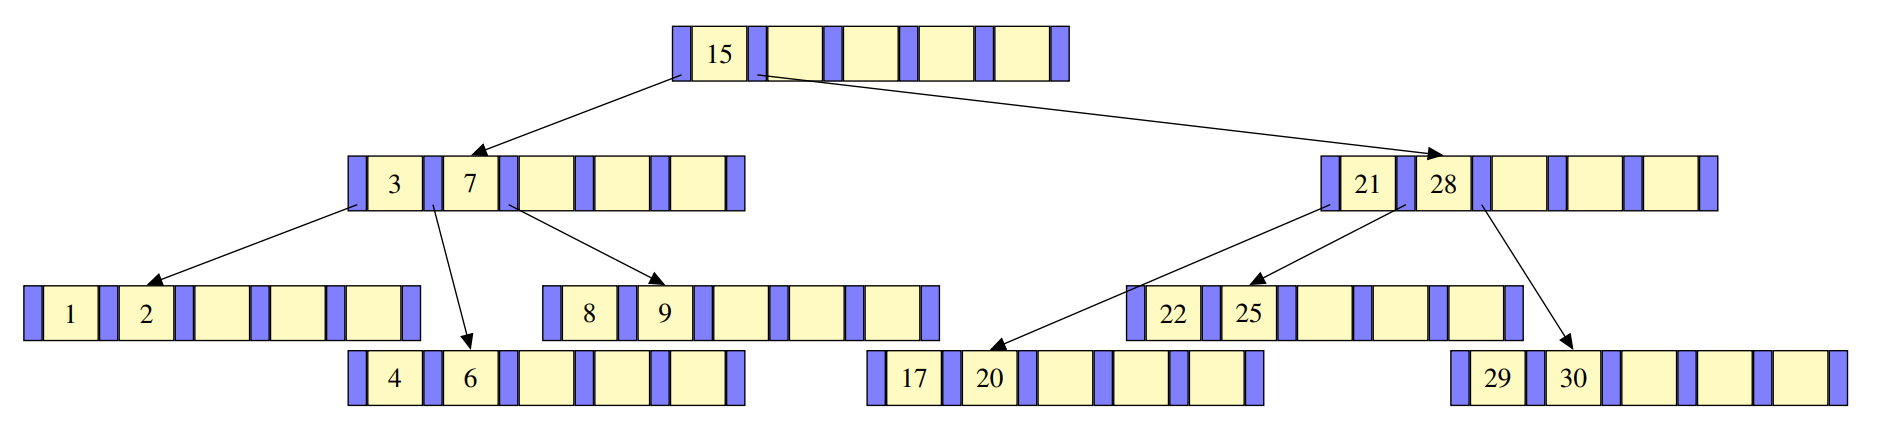
\includegraphics[width=1\textwidth]{img/btree.PNG}
    \caption{B-Tree with \(t=3\), \(N=17\), \(h=2\)}
    \label{fig:b_tree}
\end{figure}
\begin{prop}
    The height \(h\) of a B-Tree with \(N\) keys satisfies
    \begin{equation}
        h \leq \log_{t} \frac{N+1}{2}
    \end{equation}
    \begin{proof}
        The root node contains at least one key and every other node contains at least \(t-1\) keys. When maximum height is considered, the number of elements in each node is minimized, thus the root as degree 2 and every other node has degree \(t\).\\
        Because of that we will have \(2 t^{i-1}\) nodes at level \(i\) so the number of keys in the tree is:
        \begin{equation} \label{eq:height_b_tree}
            N \geq 1 + (t-1)\sum_{i=1}^{h} 2t^{i-1} = 1 + (t-1) 2 \frac{t^h - 1}{t - 1} = 2t^h - 1
        \end{equation}
        \noindent Which implies \(t^h \leq \frac{N+1}{2}\) and taking the logarithm we get:
        \begin{equation}
            h \leq \log_{t} \frac{N+1}{2}
        \end{equation}
    \end{proof}
\end{prop}
\begin{teo}
    The number of keys \(N\) in a B-Tree of height \(h\) and minimum degree \(t\) satisfies the following inequality:
    \begin{equation}
        2t^h - 1 \leq N \leq (2t)^{h+1} - 1
    \end{equation}
    \begin{proof}
        The first inequality is already demonstrated in the previous proposition (Equation \ref{eq:height_b_tree}).
        \noindent For the second inequality we can use the fact that the maximum number of keys in a B-Tree is obtained when every node has \(2t-1\) keys. In this case, the number of keys in each node is maximized, and we have:
        \begin{equation}
            N \leq (2t-1) \sum_{i=0}^{h} (2t)^i = (2t-1) \frac{(2t)^{h+1} - 1}{(2t) - 1} = (2t)^{h+1} - 1
        \end{equation}
    \end{proof}
\end{teo}
\begin{es}
    How many elements can be stored in a B-Tree of height \(h=3\) and minimum degree \(t=100\)? (Give a range for \(N\) using the previous theorem).
\end{es}
\begin{defin}[Loading factor]
    The loading factor \( \alpha \) of a B-tree is the ratio between the number of keys present in the tree and the total number of keys that could be allocated in it, i.e., \( (2t - 1)g \), where \( g \) is the number of nodes in the tree.
\end{defin}
\begin{prop}
    The average loading factor of a B-tree is approximately \(\alpha \approx 0.7 \).  
\end{prop}
\section{Searching on B-Trees}
Let \(r\) be the root of the tree, \(k\) the key to search. The algorithm works as follows:
\begin{algorithm}[H]
    \caption{Search(\textbf{key} \(k\), \textbf{root} \(v\))}
    \label{alg:b_tree_search}
    \begin{algorithmic}[1]
    \State \( i \gets 0 \)
    \While{$i < c(v)$ and $k > k_{i+1}$}
        \State \( i \gets i+1 \)
    \EndWhile
    \If{$i < c(v)$ and $k_{i+1} = k$}
        \State \Return \( \text{elem}_i \)
    \Else
        \If{$v$ is a leaf}
            \State \Return \texttt{null}
        \Else
            \State \Return \textsc{Search}(\( i \)-th child of \( v \), \( k \))
        \EndIf
    \EndIf
    \end{algorithmic}
\end{algorithm}
\noindent
Since every recursive call goes to the next level of the tree the algorithm has \(O(\log_t N)\) complexity. The biggest advantage is gained when each node of the B-Tree occupises exactly a page of the external memory. This happens when \(t = c B, c \in \mathbb{N}\) and in this case the number of I/O operations corresponds to the height of the tree.
\begin{equation}
    T(N,M,B) \in O(\log_t N) \approx O(\log_B N) 
\end{equation}
\noindent
The number of elementar operations is influenced by the fact that in each node we need to look for the key \(k\), since the keys are sorted this has \(O(log_2 t)\) complexity. The total work complexity is:
\begin{equation}
    W(N,M,B) \in O(\log_t N \cdot \log_2 t) \approx O(\log_B N \cdot \log_2 B) = O\left(\frac{\log_2 N}{\log_2 B} \cdot log_2 B\right) = O(\log_2 N)
\end{equation}
\section{Insertion on B-Trees}
The instertion of an element \(e\) with key \(k\) is performed by searching \(k\) in the tree and inserting \(k\) in the right leaf \(f\). The research has to fail because in B-Trees every key must be unique. The algorithm works as follows:
\begin{itemize}
    \item if the leaf \(f\) is not full, insert \(k\) in \(f\) and stop;
    \item if the leaf \(f\) is full, \textbf{split} it into two leaves \(f_1\) and \(f_2\) and insert the median key in the parent node of \(f\) and set the two pointers to refer to \(f_1\) and \(f_2\). Since each leaf contains at most \(2t-1\) elements when it's full the median key is the \(t\)-th one. If the parent node is also full the spilit is repeated recursively until the root is reached. If the root is split a new root is created and the height of the tree increases by one.
\end{itemize}
\noindent The split operation works as follows:
\begin{itemize}
    \item create a new node \(g\) and copy the last \(t\) keys from \(f\) to \(g\);
    \item leave the first \(t-1\) keys in \(f\);
    \item put the t-th key in the parent node of \(f\) and set the two pointers to refer to \(f\) and \(g\);
\end{itemize}
The split has work complexity \(W(N,M,B) = O(t) \approx O(B)\) e transfer complexity \(T(N,M,B) = O(1)\). The insert requires, in the worst case scenario, to perform the split operation \(h\) times, where \(h\) is the height of the tree. This brings the total complexity of the insertion to:
\begin{equation}
    W(N,M,B) = O(t \; log_t N)
\end{equation}
\begin{equation}
    T(W,N,B) = O(log_t N)
\end{equation}
\section{Deletion from B-Trees}
The deletion of a key \(k\) from a B-Tree is performed by searching for \(k\) in the tree. The algorithm works as follows. If \(k\) is \textbf{not in a leaf node}, replace \(k\) with his successor \(k'\) recursively and delete \(k'\) from the leaf node.
\begin{defin}[Almost-empty]
    A leaf \(f\) is almost empty if it contains at least \(t\) keys.
\end{defin}
\noindent
If \(k\) is in a leaf node \(f\) and \(f\) is \textbf{not almost empty} we can simply delete \(k\) from \(f\). If \(f\) is almost empty we have to do the following:
\begin{itemize}
    \item if the left or the right sibling of \(f\) is not almost empty we redistribute the keys between \(f\) and the sibling. We will also need to modify the separating key in the parent node;
    \item if both siblings are almost empty we merge \(f\) with one of the siblings (this operation is called \textbf{fuse}). To do so we add to one of the sibling the keys of \(f\) and the separating key in the parent node. The parent node will lose one key and one pointer. If the parent node is almost empty we repeat the operation recursively until we reach the root. If the root becomes empty we remove it and decrease the height of the tree by one.
\end{itemize}
\noindent So in the worst case scenario the delete will have to perform the fuse operation \(h\) times, where \(h\) is the height of the tree. The work complexity and the transfer of the delete operation are:
\begin{equation}
    W(N,M,B) = O(t \; log_t N)
\end{equation}
\begin{equation}
    T(W,N,B) = O(log_t N)
\end{equation}
\begin{es}\label{ess}
    Considering a B-Tree of minimum degree \(t=3\), insert the following keys: 11, 29, 40, 37, 66, 51, 46, 80, 24, 12, 53, 98, 85, 59, 38, 45, 22, 65, 42, 72, 93, 43, 70, 83, 58, 95, 74, 48, 41, 50, 63, 86. A solution is provided in Figure \ref{fig:b_tree_insert}.
\end{es}
\begin{figure}
    \centering
    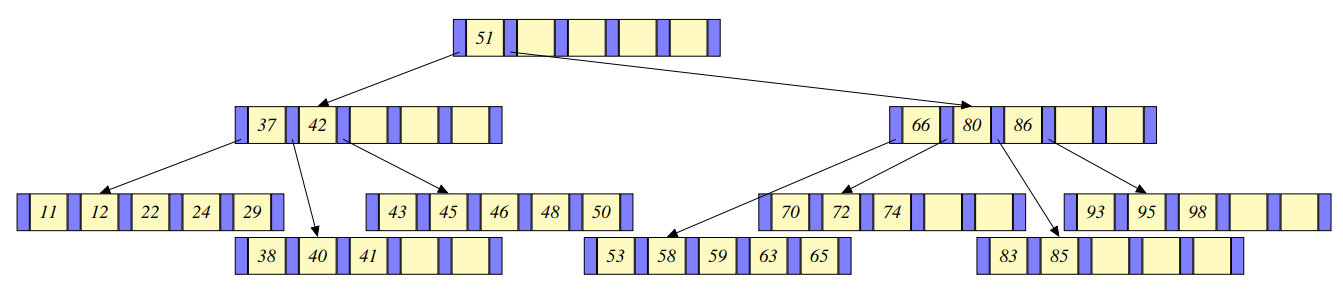
\includegraphics[width=1\textwidth]{img/sol.PNG}
    \caption{Solution to Exercise \ref{ess}}
    \label{fig:b_tree_insert}
\end{figure}

\chapter{B+ Trees}
In \textbf{B-trees}, leaf node pointers are null, wasting space. To optimize this, we can \textbf{eliminate pointers in leaves} and store more keys, increasing storage efficiency without changing the tree height.  
\smallskip \\Similarly, increasing space in \textbf{internal nodes} allows for more pointers, leading to \textbf{fewer levels} and a shorter tree height. Since full records are usually stored in B-trees, keeping them only in the \textbf{leaves} while storing only \textbf{keys in internal nodes} further reduces tree height.  
\smallskip \\Additionally, \textbf{linking leaves in a bidirectional chain} optimizes \textbf{range queries}, as elements remain sorted. This structure is called a \textbf{B+ tree}, an improved version of the B-tree, ideal for \textbf{primary indexing} without duplicate keys.  

\begin{defin}[B+ Tree] A \textbf{B+ tree} of minimum degree \( t \) for a collection of records \( C \) with key \( k \), which does not allow duplicates, is a search tree with the following properties:
\begin{enumerate}
    \item Each node occupies a block.
    \item All leaves are at the same depth and are linked by a bidirectional chain.
    \item A non-root internal node contains \( \delta \in [t - 1, 2t - 1] \) distinct keys, \( \delta + 1 \) pointers to children, and a pointer to its parent.
    \item A non-root leaf contains \( \beta \in [b, 2b] \) records ordered by key, two pointers to the previous and next leaves in the chain, and a pointer to its parent.
    \item The root, if it is not a leaf, contains \( \delta \in [1, 2t -1] \) keys and \( \delta +1 \) pointers to children.  
          If it is a leaf, it contains \( \beta \in [0, 2b] \) records ordered by key.
    \item The leaves, read from left to right, contain all records of \( C \) sorted by key.
    \item Given an internal node \( v \) with keys \( k_1 < k_2 < \dots < k_{\delta} \) and children \( w_1, w_2, \dots, w_{\delta+1} \), the following holds:
    \begin{itemize}
        \item The subtree rooted at \( w_1 \) contains a subset of records with keys smaller than \( k_1 \).
        \item The subtree rooted at \( w_i \), for \( 1 < i \leq \delta \), contains records with keys in the interval \( [k_{i-1}, k_i) \).
        \item The subtree rooted at \( w_{\delta+1} \) contains records with keys greater than or equal to \( k_{\delta} \).
    \end{itemize}
\end{enumerate}
\noindent The parameters \( t \) and \( b \) are defined as follows:
\begin{itemize}
    \item \( t \) is the largest positive integer such that a block can contain \( 2t - 1 \) keys and \( 2t + 1 \) pointers (including the pointer to the parent node).
    \item \( b \) is the largest positive integer such that a block can contain \( 2b \) records and 3 pointers to other blocks (parent, left sibling, and right sibling).
\end{itemize}
\noindent
From this definition, it follows that the same key cannot appear more than once in internal nodes.
\end{defin}
\begin{prop}\label{prop:b+_tree}
    A B+ tree with parameters \( t,b \) of height \(h\) has a number of elements \(N\) that satisfies
    \begin{equation}
        2t^{h-1}b \leq N \leq (2t)^h 2b
    \end{equation}
\end{prop}
\begin{teo}
    A B+ tree with parameters \( t,b \) containing \( N \) records has height \(h\) such that
    \begin{equation}
        h \in \Theta \left( 1 + \log_t \left\lceil \frac{N}{b}\right\rceil  \right)
    \end{equation}
\end{teo}
\begin{proof}
    The proof is similar to the one for B-trees. Let \( h \) be the height of the tree (thus, the levels range from \( 0 \) to \( h \), making a total of \( h + 1 \) levels).  
    If \( N \leq 2b \), there is only the root node, resulting in a single level. \\
    Now, suppose \( N > 2b \). Since the root has at least 2 children and each internal node has at least \( t \) children,  
    at level \( i \) of the tree, there are at least \( 2t^{i-1} \) nodes for \( 1 \leq i \leq h \).  
    Thus, the tree has at least \( 2t^{h-1} \) leaves.  
    Since each leaf contains at least \( b \) records, we obtain:  
    \[
    N \geq 2t^{h-1} \cdot b
    \]
    which leads to:
    \[
    h - 1 \leq \log_t \frac{N}{2b}
    \]
    On the other hand, every internal node, including the root, has at most \( 2t \) children, so the maximum number of leaves is \((2t)^h\)
    Since each leaf contains at most \( 2b \) records, we get:  
    \[
    N \leq (2t)^h \cdot 2b
    \]
    which simplifies to:
    \[
    h \geq \log_{2t} \frac{N}{2b}
    \] 
    thus, we finally obtain:
    \[
    \frac{\log_t \frac{N}{b} - \log_t 2}{\log_t 2t} \leq h \leq 1 + \log_t \frac{N}{b} - \log_t 2
    \]
    Since all terms except \( \log_t \frac{N}{b} \) are constants, the thesis follows.
\end{proof}
\begin{es}
    How many elements can be stored in a B+ tree of height \(h=3\) and parameters \(t=3, b=2\)? (Give a range for \(N\) using Preposition \ref{prop:b+_tree}).
\end{es}
\section{Searching on B+ Trees}
Searching on B+ Trees is similar to searching on B-Trees. The only difference is that in B+ Trees, the search is performed only in the leaves.\\
Given a key value \( k \), the goal is to find the leaf (if it exists) that contains the record with key \( k \).  
The method involves traversing the tree, following for each node the subtree \( w_i \) such that:
\[
k_{i-1} \leq k < k_i
\]
\noindent where we assume \( k_0 = -\infty \) and \( k_{\delta+1} = +\infty \), for \( i = 1, \dots, \delta + 1 \).  
Upon reaching a leaf \( u \), we search for \( k \) among its records.  
If \( k \) is found, the associated record is returned; otherwise, the search ends unsuccessfully.  \\
Since each node is stored in a single page, the number of I/O operations corresponds to the number of levels in the tree:
\begin{equation}
T(N, t, b) \in \Theta\left( 1 + \log_t \left\lceil \frac{N}{b} \right\rceil \right)
\end{equation}
\noindent
The I/O complexity decreases as \( t \) and \( b \) increase, meaning larger page sizes improve performance. \\
Regarding the number of elementary operations, searching within a page can be done using \textit{binary search},  
which requires at most \( \log_2 (2t) \) operations in internal nodes and \( \log_2 (2b) \) operations in leaves.  
Since there are \( h \) levels of internal nodes, we obtain:
\begin{equation}
W(N, t, b) \in O \left( \log_2 (2t) \cdot \log_t \left\lceil \frac{N}{b} \right\rceil + \log_2 (2b) \right)
\end{equation}
\noindent
which simplifies to:
\begin{equation}
O \left( \log_2 (2t) \cdot \frac{\log_2 \left\lceil \frac{N}{b} \right\rceil}{\log_2 t} + \log_2 (2b) \right) = O \left( \log_2 \left\lceil \frac{N}{b} \right\rceil + \log_2 b \right)
\end{equation}
\section{Insertion on B+ Trees}
The insertion of a record \( r \) with key \( k \) involves an unsuccessful search that identifies the leaf \( u \) where \( r \) should be inserted.  
If \( u \) contains \textbf{fewer} than \( 2b \) records, \( r \) is inserted in order among the existing records.  
However, if \( u \) already contains \( 2b \) records, a \textit{leaf split} is required.
\noindent
Let \( r_1, \dots, r_{2b+1} \) be the ordered records in \( u \), including \( r \).  
The node \( u \) is split into two nodes \( u_1 \) and \( u_2 \):  
\begin{itemize}
    \item \( u_1 \) contains records \( r_1, \dots, r_b \)  
    \item \( u_2 \) contains records \( r_{b+1}, \dots, r_{2b+1} \)  
    \item The key \( k_{b+1} \) (median value) of record \( r_{b+1} \) is inserted into the parent of \( u \) with pointers to \( u_1 \) and \( u_2 \).  
\end{itemize}
If \( u \) was the \textit{root}, a new root node is created containing \( k_{b+1} \) and pointers to \( u_1 \) and \( u_2 \).  
If the \textit{parent of \( u \)} was already full (i.e., contained \( 2t - 1 \) keys), it must also be split like we saw for B-Trees.  
This splitting process may propagate up to the root, so the number of I/O operations is proportional to the height of the tree:
\begin{equation}
T(N,t,b) \in \Theta \left( 1 + \log_t \left\lceil \frac{N}{b} \right\rceil \right)
\end{equation}
\noindent
Regarding \textit{work complexity}, each node split requires moving \textit{half of its data}, i.e.,  
\begin{itemize}
    \item \( O(t) \) operations for \textit{internal nodes}  
    \item \( O(b) \) operations for \textit{leaves}  
\end{itemize}
\noindent Thus, the total work complexity is:
\begin{equation}
W(N,t,b) \in O \left( b + t \cdot h \right) = O \left( b + t \log_t \left\lceil \frac{N}{b} \right\rceil \right)
\end{equation}
\section{Deletion on B+ Trees}
The deletion of a record \( r \) with key \( k \) requires first locating the leaf \( u \) where \( r \) is stored. The record \( r \) is then removed. If \( u \) is the \textbf{root} or still contains more than \( b \) records after deletion, the process terminates. Otherwise there would be only b-1 records in \(u\), let \( r_1, \dots, r_{b-1} \) be the remaining records in \( u \).
\\If the \textbf{right sibling} (or left sibling) of \( u \), denoted as \( u' \), contains more than \( b \) records, a \textbf{redistribution} is performed. Let \( v \) be the parent of \( u \), and let \( \hat{k} \) be the key that separates \( u \) and \( u' \). Records are redistributed between \( u \) and \( u' \), and \( \hat{k} \) in \( v \) is updated accordingly.
\\If \( u' \) has exactly \( b \) records, a \textbf{merge} is performed. All records from \( u' \) are moved into \( u \), and the separator key \( \hat{k} \) is removed from \( v \). If \( v \) still contains at least \( t - 1 \) keys or is the root, the process stops. Otherwise, if \( v \) now has fewer than \( t - 1 \) keys, the procedure recurses upwards.
\\The number of I/O operations required is proportional to the height of the tree:
\begin{equation}
T(N,t,b) \in \Theta \left( 1 + \log_t \left\lceil \frac{N}{b} \right\rceil \right)
\end{equation}
\noindent
Since each merge or redistribution involves shifting data, the \textbf{work complexity} is determined by:
\begin{itemize}
    \item \( O(t) \) operations for \textit{internal nodes}.
    \item \( O(b) \) operations for \textit{leaves}.
\end{itemize}
\noindent
Thus, the total complexity is:
\begin{equation}
W(N,t,b) \in O \left( b + t \log_t \left\lceil \frac{N}{b} \right\rceil \right)
\end{equation}
\section{Range query on B+ Trees}
The search for all records with keys in the interval \([k_1, k_2]\) begins by locating the leaf containing a record with key \( k_1 \).
Once found, the search continues to the right, scanning successive leaves to collect all records with keys within \([k_1, k_2]\). Let \( R \) be the number of records retrieved.  
Since the leaves are linked by a bidirectional chain, scanning successive leaves is very efficient. Let \(r\) be a record in a leaf \(f\), the operation \textbf{next}(\(r\)) is performed in \(O(1)\) time. If the \(r\) is the rightmost element in \(f\) is successor is the first element of the next leaf otherwise is the next element in the same leaf.\\
The I/O cost consists of the search operation plus accessing the subsequent leaves, yielding: \\  
\begin{equation}
T(N,t,b) \in \Theta \left( 1 + \log_t \left\lceil \frac{N}{b} \right\rceil + \left\lceil \frac{R}{b} \right\rceil \right)  
\end{equation}
For the work complexity, the search requires: \\  
\begin{equation}  
W(N,t,b) \in O \left( \log_t \left\lceil \frac{N}{b} \right\rceil + \log b + R \right)  
\end{equation}
\begin{es}
    Insert the following keys into a B+ tree with parameters \( t=3 \) and \( b=2 \):  
    \\55, 65, 81, 11, 69, 47, 45, 27, 71, 49, 80, 31, 86, 36, 10, 38, 84, 37, 89, 20.
\end{es}

\chapter{Hash tables}
In general techniques based on comparing keys have at best \(O(\log n)\) complexity, with \(n\) beeing the total number of keys. There exist search techniques that do not rely on comparisons and can achieve \textbf{constant-time} complexity, meaning the time required is independent of the number of data items. These methods are based on transforming keys into addresses. 

If we had distinct integer keys ranging from $1$ to $N$, we could store the data with key $i$ in the $i$-th position of a table. In this way, data access would be immediate.

\textbf{Hashing} methods generalize this very particular situation to cases in which the keys do not have such ideal properties. The first step of a hash-based search consists of computing a \textit{hash function} that transforms the search key into an address within the table where data is stored. That is, a function
\[
h : K \rightarrow \{0, 1, \dots, m - 1\}
\]
where $K$ is the set of keys and $\{0, 1, \dots, m - 1\}$ are the addresses of the table positions.

Ideally, different keys $k_1 \ne k_2$ should map to different addresses $h(k_1) \ne h(k_2)$, but unfortunately, hash functions are rarely injective. As a result, two or more distinct keys may produce the same address.

When $h(k_1) = h(k_2)$ for $k_1 \ne k_2$, a {\textbf{collision}} is said to occur, and $k_1$ and $k_2$ are called {\textbf{synonyms}}. The second part of a hash-based search concerns the mechanisms used for \textbf{collision resolution}.

\subsubsection{Searching in a hash table}
Suppose we have a hash function $h$ and a collision resolution method $M$. The search for a key $k$ proceeds as follows:

\begin{enumerate}
    \item Compute $h(k)$ and check the element at that position.
    \item If the element has key $k$, the search concludes successfully. Otherwise, it is still unclear whether $k$ is absent from the table or whether a collision occurred during insertion and $k$ was stored at a different position.
    \item Apply the method $M$ to $k$; either the key is found or it is concluded that $k$ is not present.
\end{enumerate}
\noindent
If $h$ is a good hash function and produces few collisions, then most data can be accessed with a single step and comparison. In the case of collisions, if $M$ is a good resolution method, the number of accesses is very limited, and thus the overall search time remains nearly constant.
\subsubsection{Hash function}
A hash function must transform keys (typically integers or strings) into integers in the range $[0, m - 1]$, where $m$ is the number of elements in the table. A good hash function $h$ should satisfy the following properties:
\begin{enumerate}
    \item It should be easy to compute, so as not to burden the auxiliary operations related to the search;
    \item It should generate values that are uniformly distributed over the interval $[0, \dots, m - 1]$.
\end{enumerate}
\begin{defin}[Perfect hash function]
    A hash function is said to be \textbf{perfect} if it is injective, meaning that it maps distinct keys to distinct addresses. In this case, the search time is constant and equal to one access. 
\end{defin}
\noindent In general, it is not possible to construct a perfect hash function for all possible keys, this would require a very high value of \(m\). The simplest hash function for numeric values is 
\begin{equation}
    h(k) = k \mod m
\end{equation}
\noindent To deal with alphabetic strings we need to enstablish a rule to convert them into integers. For example we can consider alphabetic characters as numbers in base 26. In this case we define the hash function as follows. Let k be a string of length \(n\), \(k_i\) be the \(i\)-th character of the string, \(v(k_i)\) the corrisponding value.
\begin{equation}
    h(k) \doteq \sum_{i=0}^{n-1} v(k_i) \cdot 26^i \mod m
\end{equation}
\noindent The choice of \(m\) is very important. If \(m\) is a prime number, the distribution of the hash function is more uniform. In general, it is advisable to choose \(m\) as a prime number. This is due to the properties of the module operation.

Another widely used method for alphabetic keys is the \textbf{{folding} method}. Suppose the key is a string of 12 characters, each represented with 8 bits. We divide the key into 4 groups of 3 characters each and compute the \textit{exclusive OR (XOR)} of the four groups.
\\ A property of XOR is that each input influences the final result, which in this case is a 24-bit value that depends on all 12 characters of the original string. These 24 bits can be interpreted as a number, to which we can apply, for example, the modulo operation to obtain the final value in the range $[0, \dots, m - 1]$.
\section{Collision resolution methods}
Collesion resolution methods can be divided into two categories, those that use chained structures to memoraize synonyms and those that recompute new addresses in case of collision.
\subsubsection{Separate chaining methods}
The collision resolution method known as \textit{separate chaining} organizes the table such that its elements contain only pointers to chains. Each chain stores all the data items that are \textit{synonyms}, i.e., keys for which the hash function computed the same address — the address corresponding to the table position containing a pointer to the head of the chain.

To insert a new key $k$, one computes $h(k)$ and inserts $k$ into the chain pointed to by the entry at position $h(k)$ of the table. Searching is done in a similar way: the value of the hash function determines the chain to access, which is then traversed sequentially.

Note that this is the only case of a hash table in which it is possible to store a number of elements $n$ greater than the length $m$ of the table.
\begin{es}
    Use the separate chaining method to store the following keys in a hash table of size \(m=11\) using hash function \(h(k) = k \mod m\). \(1, 19, 5, 12, 18, 3, 8, 9, 14, 7, 16, 24, 23, 13, 27, 34, 38\). The solution is shown in Figure \ref{fig:hash_table}.
\end{es}
\begin{figure}
    \centering
    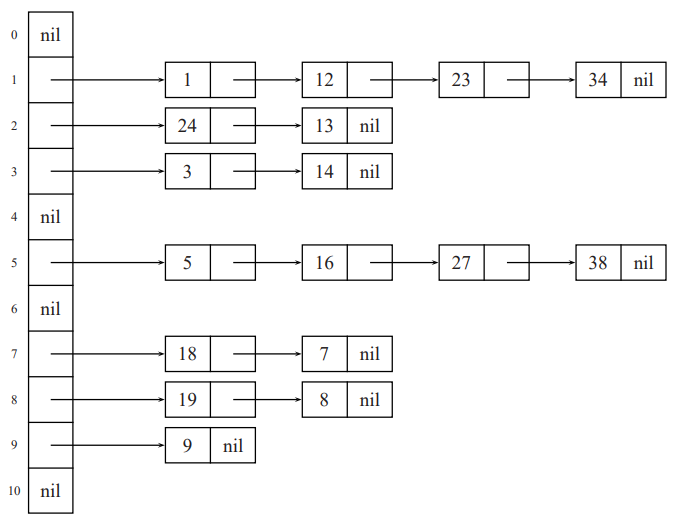
\includegraphics[width=0.8\textwidth]{img/hash_separata.PNG}
    \caption{Hash table with separate chaining method}
    \label{fig:hash_table}
\end{figure}
\subsubsection{Joined chaining methods}
A structurally simpler method, though limited by the condition $n \leq m$—is the implementation of hash tables using \textit{coalesced chaining}. In this case, each element in the table consists of two fields: one containing the key and the other an index.

Each element is inserted into the position indicated by the hash function. If that position is free, the key is placed there and the index is set to $-1$. When a collision occurs, the new key $k$ is inserted into the first available position after $h(k)$ (the table is considered circular), and the index of position $h(k)$ is updated to point to this new location.

If another synonym is inserted later, it first accesses $h(k)$ and finds it occupied. It then follows the index to the position of the first synonym and proceeds in the same way—being placed in the first free position after that, with its index linked from the previous entry.

It may happen that, when inserting a key $k_1$, the position $h(k_1)$ is already occupied by a key $k_2$ that is \textit{not} a synonym but ended up there while searching for a free position. In this case, it is preferable to replace $k_2$ with $k_1$ (so $k_1$ can be accessed in a single step) and reallocate $k_2$. This operation does not increase the number of steps required to retrieve $k_2$.
\begin{es}
    Use the joined chaining method to store the following keys in a hash table of size \(m=11\) using hash function \(h(k) = k \mod m\). \( 1, 19, 5, 12, 18, 3, 8, 23, 14, 7, 17\). The solution is shown in Figure \ref{fig:hash_table2}.
\end{es}
\begin{figure}
    \centering
    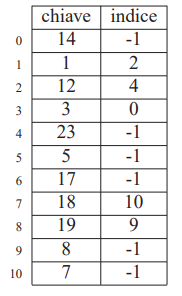
\includegraphics[scale=1]{img/hash_unita.PNG}
    \caption{Hash table with joined chaining method}
    \label{fig:hash_table2}
\end{figure}
\subsubsection{Open addressing method}
Hash methods that use chaining require additional memory to store pointers or indices. By observing the coalesced hashing method, one might consider removing the indices and instead performing a \textit{sequential search} for synonyms starting from the position $h(k)$.

This approach saves space but increases the number of comparisons required during search. An unsuccessful search ends when an empty position is encountered, so to avoid infinite loops, it is necessary to ensure that $n < m$. Moreover, the greater the number of empty slots, the faster the search can conclude. The cost of search depends in fact on the \textbf{load factor} of the hash table.
\begin{equation}
    \alpha = \frac{n}{m}
\end{equation}
\noindent The insertion with open addressing is performed as follows. Suppose that empty positions are marked with \(T[x] = -1\).
\begin{algorithm}[H]
    \caption{Insertion (\textbf{key} \(k\), \textbf{table} \(T\))}
    \begin{algorithmic}[1]
    \State \( x = h(k) \)
    \While{\(T[x] != -1\)}
        \State \( x = (x+1) \mod m \)
    \EndWhile
    \State{} \(T[x] = k\)
    \end{algorithmic}
\end{algorithm}
\begin{es}
    Use the open addressing method to store the following keys in a hash table of size \(m=19\) using hash function \(h(k) = k \mod m\). \( 1, 19, 5, 20, 18, 3, 8, 9, 14, 7, 24, 43, 39, 13, 16, 12, 62\).
\end{es}
\begin{teo}
    When the collision resolution method is open addressing, the average number of comparisons required to search for a key \(k\) in a hash table of size \(m\) with \(n\) is
    \begin{equation}
        \frac{1}{2} \left( 1 + \frac{1}{1-\alpha}\right)
    \end{equation}
    in case of success and
    \begin{equation}
        \frac{1}{2} \left( 1 + \frac{1}{(1-\alpha)^2}\right)
    \end{equation}
    in case of failure.
\end{teo}
\section{Hash in external memory}
Just like tree structures, hashing techniques can also be adapted to secondary memory and retain the same advantages and limitations observed in main memory:

\begin{enumerate}
    \item Random access \textbf{performance is better} than with tree-based structures.
    \item Key dispersion makes \textbf{any sorting operation extremely costly}.
    \item Due to the scattering of keys, range queries are not possible.
\end{enumerate}
\noindent
However, when neither sorting nor range queries are required, hash-based organization is highly efficient, typically requiring just over one access to secondary memory per search. This makes hashing very practical in real-world applications such as record storage and index management.

From a technical perspective, the main drawback of hash-based organization is its \textbf{{static nature}}: 
while tree structures can grow by adding pages as the number of keys increases, hash techniques require that the archive size be known in advance. Expanding it later involves an expensive full rehashing of the entire archive. For this reason, the most significant research on hashing in \textit{External Memory (EM)} has focused on techniques for making hash structures dynamic.
\subsection{Static hashing}
The idea behind static hashing is to use a hash function that maps the keys into the pages (\textbf{buckets}) in witch they will be stored. Untill the page is full synonyms are added sequantially in the same page, the collision resolution problem occurs when the page is full.

Let \(B\) be the number of keys that can be stored in a page, \(N\) the total number of keys. To solve the collisions there are two different approaches:
\begin{itemize}
    \item collect all the keys that cannot be stored in the designed page in \textbf{overflow pages};
    \item similar to the \textit{separate chaining method} , when a page of synonyms is full store the new synonyms in a new page linked to the previous one with a linked list.
\end{itemize}
\noindent Like in the case of main memory, the cost of searching depends on the load factor \(\alpha\) of the hash table.

To memorise the keys we need a table contaning more than \(\lceil \frac{N}{B} \rceil\) pages. In particular to have a load factor \(\alpha = 0.8\) we need at least \(\lceil 1.25 \frac{N}{B} \rceil\) pages.

The number of I/O operations required to search for a key \(k\) in a hash table of size \(m\) with \(n\) keys is, in the worst case, \(O(\lceil \frac{N}{B} \rceil)\). Although, when the hash function distributes the keys uniformly the average number of I/O operations is:
\begin{equation}
    \frac{\lceil \frac{N}{B} \rceil}{m} = \frac{\lceil \frac{N}{B} \rceil}{1.25 \lceil \frac{N}{B} \rceil} = \frac{1}{1.25}
\end{equation}
\subsection{Dynamic hashing}
To enable an archive to grow dynamically while using a hash-based organization, the technique of \textit{Dynamic Hashing} has been introduced. Suppose we have a pseudorandom function:
\begin{equation}
    \sigma : K \to [0, m - 1]
\end{equation}
which transforms keys into binary-coded integers. For any key \( k \in K \), let:
\begin{equation}   
    \sigma(k) = b^{(k)}_1 b^{(k)}_2 \ldots b^{(k)}_{\lceil \log_2 m \rceil}
\end{equation}
be the binary representation of the value obtained from \( \sigma \). The insertion of keys proceeds as follows:
\begin{itemize}
    \item Initially, a single page \( P \) is allocated, and all keys are inserted into it.
    \item When \( P \) becomes full, a second page \( Q \) is created.
    \item The keys in \( P \) are redistributed based on the first bit of their hash value:
    \begin{itemize}
        \item If \( b^{(k)}_1 = 0 \), the key remains in \( P \).
        \item If \( b^{(k)}_1 = 1 \), the key is moved to \( Q \).
    \end{itemize}
    \item The new key that caused the split is inserted into \( P \) or \( Q \), according to its first bit.
\end{itemize}
\noindent
If \( \sigma \) is a good pseudorandom function, the keys will be distributed uniformly between the two pages.

When a page becomes full again, the process is repeated, but this time the second bit of the hash value is used to determine the destination page. This process continues until all bits of the hash value are used.
Internal nodes do not contain keys but only two pointers to the pages corresponding to the two possible values of the next bit. This allows the tree to be contained in central memory, while the pages can be stored on disk. Since the entire tree can be stored in internal memory we will always need just one I/O operation to reach every key in the archive.
\begin{figure}
    \centering
    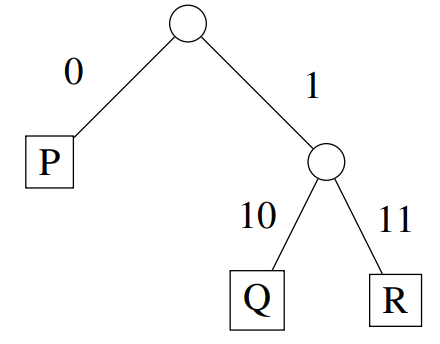
\includegraphics[scale=0.7]{img/hashdinamico.PNG}
    \caption{Dynamic hashing}
    \label{fig:dynamic_hash}
\end{figure}
\subsection{Extendible hashing, methods with directory}
The idea behind Extendible hashing is to use multiway trees instead of binary trees. This will result in a lower load factor.

To overcome the issue of underloaded pages in multi-way tries, in 1978, Fagin, Nievergelt, Pippenger, and Strong proposed a new method called \textit{Extendible Hashing}, which (almost always) requires only one or two I/O operations for search and insertion. Suppose we have a hash function 
\begin{equation}
h : K \rightarrow \{0,1,2,\ldots,m-1\}
\end{equation}
that maps keys to binary-encoded integers, where the range $m$ of the hash function is chosen to be sufficiently large.

The method uses a \textbf{{directory}}, i.e., an array of $2^d$ pointers to pages. Each key $k$ is assigned to the page pointed to by the directory location corresponding to the $d$ most significant bits of $h(k)$. The value $d$ is called the \textbf{{Global Depth}} and is initially set to the smallest value such that each page can contain at most $B$ keys. The value $d$ can be increased when that condition is no longer satisfied.

Two or more directory locations can point to the same page if the total number of keys assigned to them is less than or equal to $B$. In that case, such locations share the same page if they have the first $c$ bits of their address in common, with
\begin{equation}
0 \leq c \leq d
\end{equation}
The value $c$ is called the \textbf{Local Depth} and represents the smallest number of bits needed to distinguish a group of keys in the same page.

\begin{defin}
An \textit{extendible hash table} of order $d$ is a directory with $2^d$ references to pages, each of which can hold up to $B$ records. All records in the same page $P$ have the first $c$ bits of $h(k)$ in common. The directory contains $2^{d - c}$ pointers to page $P$, starting from the location specified by those $c$ leading bits.
\end{defin}
\noindent To maintain these properties, two key operations are required:
\begin{itemize}
  \item \textit{Page Split}: When a page overflows, it is split into two pages. The keys are redistributed between the old and new page according to the $(c+1)$-th bit, and the local depth is updated as $c \leftarrow c + 1$.
  \item \textit{Directory Doubling}: If after a split we have $c = d$, it becomes necessary to double the size of the directory by increasing $d$ by one, thus expanding from $2^d$ to $2^{d+1}$ references to pages.
\end{itemize}
It is important to note that no page of the archive is modified during the doubling of the directory, except for the one that caused the overflow.

The deletion of an element can be performed in a similar way. When two blocks with the same local depth $c$ contain elements whose hash addresses share the same $c - 1$ most significant bits and their combined number of elements can fit into a single block, then their elements are merged into a single block with local depth $c - 1$. The total size of the two blocks being merged must be sufficiently less than $B$ in order to avoid an immediate need for a split upon subsequent insertions.

The directory is halved (and $d$ is decremented by 1) when all local depths are less than the current value of $d$.
\begin{prop}
    The extendible hash table, consisting of a set of keys, depends only on the values of the keys and not on the order in which the keys are inserted.
\end{prop}
\begin{teo}
    The expected number of pages required to store $n$ elements is asymptotically equal to
    \begin{equation}
    \frac{n}{\ln(2)} \approx \frac{n}{0.69}.
    \end{equation}
    Since \(n = \frac{N}{B}\) is the minimum number of pages needed to store \(N\) elements the load factor is approximately \(\alpha = 0.69\) and the total number of pages is 1.44 times the minimum number of pages needed.
\end{teo}
It's also important to note that the directory is an array of links. If it all fits in RAM then the cost of searching will be \(T(N,M,B) = 1\), if not a second evel can be added bringing the cost to \(T(N,M,B) = 2\).
\section*{Methods without directory}
As we saw a disadvantage of the extendible hashing method is that the directory can be very large and if it doesn't fit in RAM a second I/O operation is needed to access it. To overcome this problem, we can use a method that doesn't require a directory. Two possible techniques to achieve this are \textbf{virtual hashing} and \textbf{linear hashing}.
\subsection{Virtual hashing}
Virtual hashing is based on the following theorem.
\begin{teo}
    Given an integer $k$ and an integer divisor $d$, if $k \bmod d = r$, then
    \begin{equation}
        k \bmod 2d = r \quad \text{or} \quad r + d.
    \end{equation}
\end{teo}
\noindent
Let \(h: K \to \{0,1,2,\dots,m-1\}\) with \(m>>\). We define
\begin{equation}
    h_0 : \mathbb{N} \to \{0,1,2,\dots,d-1\}, \; h_0(k) = h(k) \mod d
\end{equation}
where \(d \in \mathbb{P}\) is a small prime number. Virtual hashing works as follows.

Initially keys are inserted in \(d\) pages of the archive using the function \(h_0(k)\). When a page \(p\) overflows, a re-hashing of the keys is performed using the function
\begin{equation}
    h_1(k) = h(k) \mod 2d
\end{equation}
wich distributes the keys between the page \(p\) and the page \(p+d\). The page \(p+d\) is created only if it is needed. In this way the archive doubles its number of pages from \(d\) to \(2d\).
\end{document}
